\documentclass[12pt,a4paper]{report}

% Packages
\usepackage[utf8]{inputenc}
\usepackage{setspace}
\usepackage{geometry}
\usepackage{hyperref}
\usepackage{graphicx}
\usepackage{titlesec}
\usepackage{amsmath} 
\usepackage{amssymb}
\usepackage{booktabs}
\usepackage{float}

\usepackage{tikz}
\usetikzlibrary{arrows.meta, calc, positioning, patterns, fadings}

\tikzstyle{block} = [draw, fill=white, rectangle, 
    minimum height=3em, minimum width=6em]
\tikzstyle{sum} = [draw, fill=white, circle, node distance=1cm]
\tikzstyle{input} = [coordinate]
\tikzstyle{output} = [coordinate]
\tikzstyle{pinstyle} = [pin edge={to-,thin,black}]

\onehalfspacing
\geometry{margin=1in}

\titleformat{\chapter}[hang]
  {\normalfont\huge\bfseries}
  {\thechapter.}
  {1em}
  {}

\begin{document}

\title{Product Sequencing on a Mixed-Model Assembly Line using Deep Learning}
\author{Christoffer Lindkvist}
\date{\today}
\maketitle

\begin{abstract}
A Mixed-Model Assembly Line (MMAL) manufactures different product variants on a single line, where variations in tasks can create imbalances across workstations. When several labour-intensive models appear consecutively, stations may exceed their capacity, leading to overloads that require halting the entire line. This challenge is formalized as the Product Sequencing Problem, an NP-hard optimization task traditionally managed by rule-based heuristics or human intuition.

This thesis investigates the viability of Deep Learning for solving this problem by emulating valid scheduling logic. We adapt and compare three Neural Network architectures: the \textbf{Sequence-to-Sequence (Seq2Seq)} model and the \textbf{Transformer} (originally derived from Natural Language Processing), alongside the \textbf{Pointer Network} (designed for combinatorial optimization). To overcome the limitations of inconsistent historical records, the models are trained on high-fidelity synthetic data generated via a constructive "solved puzzle" algorithm, which serves as a collision-free ground truth.

The models are evaluated on their ability to minimize station overlaps in permuted sequences. Results demonstrate that the \textbf{Transformer} architecture significantly outperforms the recurrent models, achieving a \textbf{93\% reduction in overlaps} on unseen test data, compared to approximately 72--75\% for the RNN-based approaches. These findings suggest that attention-based mechanisms are superior in capturing the global context required for complex constraint satisfaction in manufacturing.
\end{abstract}

\chapter*{Acknowledgements} 
Funding: Vinnova grant 2023-00970 (EUREKA ITEA4 ArtWork), Vinnova grant 2023-00450 (Arrowhead fPVN, Swedish
funding), and KDT JU grant 2023-000450 (Arrowhead fPVN,
EU funding).


\tableofcontents

\chapter{Introduction}
\section{Background}
This thesis addresses machine learning applied to the Product Sequencing Problem, an NP-Hard optimization problem which arises in the planning of mixed-model assembly lines \cite{ref6}. Traditionally, product sequences are determined manually by management staff, relying primarily on tacit knowledge accumulated through experience. While this often produces feasible solutions with relatively few scheduling conflicts, it remains ad hoc and sporadic. 

The main constraint for this problem is that the assembly line moves synchronously, if a single station exceeds its cycle time, often depicted as an overlap (see \ref{chap:overlap}), then the \textit{entire} assembly line halts. Thus, the goal of this thesis is to minimize the number of production halts.

The methods used in assembly today are strictly rules-based, and due to a large number of rules that have accumulated over the years a lot of these subtleties can prove highly restrictive in search of better solutions. 

\section{Research Problem}
Current approaches in practice rely entirely on human expertise and tacit knowledge, which limits scalability and consistency. If this knowledge could be systematically emulated using a model that mimics historical sequencing data, and in effect tacit knowledge, it may provide stronger starting points for any given adjustments to be made later on. Consequently, switching from a strictly rules-based to a time-based approach can help reduce the number of station overloads (\ref{chap:overlap}), and conflicts.

\clearpage 
\section{Objectives}
\label{sec:objectives}

The primary objectives of this thesis are:

\begin{enumerate}
    \item \textbf{Deep Learning Framework Design:} To design a supervised learning framework capable of emulating expert scheduling logic. Due to the scarcity of consistent historical records, this involves training on high-fidelity synthetic data generated via a constructive "solved puzzle" heuristic to represent valid, collision-free ground truths, see \ref{sub:datagen}.

    \item \textbf{Architectural Adaptation:} To adapt architectures originally designed for Natural Language Processing (Sequence-to-Sequence, Transformer) to the domain of combinatorial optimization. This includes modifying them to handle continuous feature vectors and enforcing permutation constraints via pointer mechanisms.

    \item \textbf{Comparative Evaluation:} To investigate and compare the performance of Recurrent versus Attention-based architectures in resolving the Product Sequencing Problem, specifically measuring their ability to minimize station overlaps, see \ref{chap:overlap}.

\end{enumerate}

\section{Visualization of the Problem}

The user interface (UI) will visualize the flow of the assembly line along two axes: one representing stations and one representing clockcycles. A clockcycle is defined as the time required for an item to move from one station to the next. In the visualization, items are displayed in a way that reflects the relative duration of processing at each station. In \autoref{fig:assembly}, this is illustrated by stretching items along the timeline to better represent the clockcycles. Note that a clockcycle is an arbitrary unit of time and does not correspond to real-world durations. For the purpose of this thesis, one clockcycle is defined as the time it takes for an arbitrary item $X$ to move from station $S_n$ to station $S_{n+1}$. 

Each entry, whose size represents the time it needs to complete its cycle, may borrow time from a previous or upcoming station, this is refered to as the \textit{"drift area"} (see \ref{chap:drift}). Unfortunately, this is where the problems related to the Mixed-Model Assembly Lines start to arise. If time-intensive items are placed consecutively, we will experience an overlap, as the time-allocations will not fit given the constraints of the station and drift areas.

\begin{figure}[ht]
    \centering
    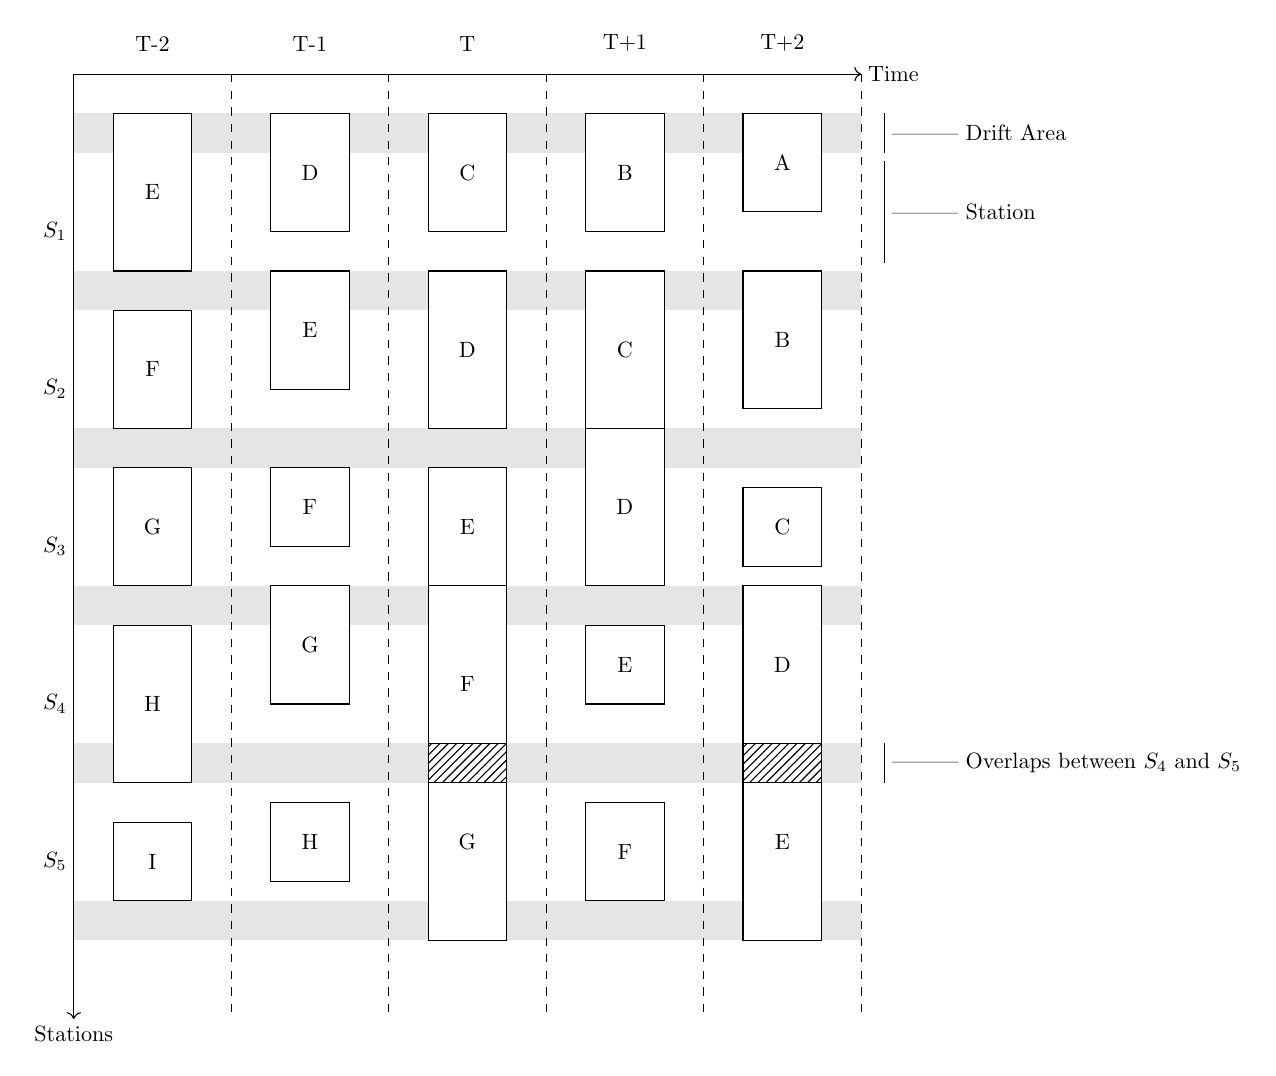
\begin{tikzpicture}[scale=1, every node/.style={scale=0.8, inner sep=3pt}]

        \foreach \y in {-1,-3,-5,-7,-9, -11} {
            \fill[gray!20] (0,\y+0.5) rectangle (10,\y);
        }

        \draw[->] (0,0) -- (10,0) node[right]{Time};
        \draw[->] (0,0) -- (0,-12) node[below]{Stations};

        \foreach \y/\name in { -2/$S_1$, -4/$S_2$, -6/$S_3$, -8/$S_4$, -10/$S_5$ } {
            \node[left] at (0,\y) { \name };
        }
        \draw[fill=white] (0.5,-9.5) rectangle (1.5,-10.5) node[midway]{I};

        \draw[fill=white] (0.5,-7) rectangle (1.5,-9) node[midway]{H};
        \draw[fill=white] (2.5,-9.25) rectangle (3.5,-10.25) node[midway]{H};

        \draw[fill=white] (0.5,-5) rectangle (1.5,-6.5) node[midway]{G};
        \draw[fill=white] (2.5,-6.5) rectangle (3.5,-8) node[midway]{G};
        \draw[fill=white] (4.5,-8.5) rectangle (5.5,-11) node[midway]{G};

        \draw[fill=white] (0.5,-3) rectangle (1.5,-4.5) node[midway]{F};
        \draw[fill=white] (2.5,-5) rectangle (3.5,-6) node[midway]{F};
        \draw[fill=white] (4.5,-6.5) rectangle (5.5,-9) node[midway]{F};
        \draw[fill=white] (6.5,-9.25) rectangle (7.5,-10.5) node[midway]{F};

        \draw[fill=white] (0.5,-0.5) rectangle (1.5,-2.5) node[midway]{E};
        \draw[fill=white] (2.5,-2.5) rectangle (3.5,-4) node[midway]{E};
        \draw[fill=white] (4.5,-5) rectangle (5.5,-6.5) node[midway]{E};
        \draw[fill=white] (6.5,-7) rectangle (7.5,-8) node[midway]{E};
        \draw[fill=white] (8.5,-8.5) rectangle (9.5,-11) node[midway]{E};

        \draw[fill=white] (2.5,-0.5) rectangle (3.5,-2) node[midway]{D};
        \draw[fill=white] (4.5,-2.5) rectangle (5.5,-4.5) node[midway]{D};
        \draw[fill=white] (6.5,-4.5) rectangle (7.5,-6.5) node[midway]{D};
        \draw[fill=white] (8.5,-6.5) rectangle (9.5,-8.5) node[midway]{D};

        \draw[fill=white] (4.5,-0.5) rectangle (5.5,-2) node[midway]{C};
        \draw[fill=white] (6.5,-2.5) rectangle (7.5,-4.5) node[midway]{C};
        \draw[fill=white] (8.5,-5.25) rectangle (9.5,-6.25) node[midway]{C};

        \draw[fill=white] (6.5,-0.5) rectangle (7.5,-2) node[midway]{B};
        \draw[fill=white] (8.5,-2.5) rectangle (9.5,-4.25) node[midway]{B};

        \draw[fill=white] (8.5,-0.5) rectangle (9.5,-1.75) node[midway]{A};

\draw[pattern=north east lines, pattern color=black] (4.5,-8.5) rectangle (5.5,-9) node[midway]{};
        
\draw[pattern=north east lines, pattern color=black] (8.5,-8.5) rectangle (9.5,-9) node[midway]{};

        \foreach \x/\label in {2/T-2, 4/T-1, 6/T, 8/T+1, 10/T+2} {
            \draw[dashed] (\x,0) -- (\x,-12);
            \node[above] at (\x-1,0.2) {\label};
        }

        \draw (10.3,-0.5) -- (10.3,-1) node[midway,right]{|---| Drift Area };
        \draw (10.3,-1.1) -- (10.3,-2.4) node[midway,right]{|---| Station };

        \draw (10.3,-8.5) -- (10.3,-9) node[midway,right]{|---| Overlaps between $S_4$ and $S_5$};


    \end{tikzpicture}
    \caption{Assembly Line Example with Uniform Station and clockcycles}
    \label{fig:assembly}
\end{figure}

    Issues in visualizing this way start to appearing when we start to consider that different stations $S_n$ and $S_m$ may take different times to complete. If we then step a clockcycle for each possible item, then we can never keep our items in sync. The main issue is that if we compare the station $S_n$ and $S_m$, then we'll see that each station have a different time to finish, then the clockcycle system will not be perfect or even realistic as stations with differing times will each finish in different times and thus an item $X$ might make it to the station $S_{n+2}$ from $S_n$ in the same time it takes item $Y$ to make it to $S_{m+1}$ from $S_{m}$.

Thus we find the difficulty in displaying it properly in an intuitive graphical user interface. If we wish to display each station as uniform sizes, then we also have to stretch the items to make up for it visually. But doing this we have no intuitive way of knowing that $S_4$ could be 200 seconds long in real life, while $S_3$ could be 300. \textit{As luck would have it, each station in this specific case are each roughly 7 minutes long, 700cmin}, thus we will not run into any major desync problems using clockcycles on these stations.

Between each station lies a buffer zone refered to a "drift area". A drift area in this case is a transitional area between any given station $S_n$ and $S_{n+1}$. Both of the stations can borrow time from each other within this area, but only one station may utilize that area at the time. This proves useful to help fit items that take longer on some stations onto the assembly line, but these conveniences which at first glance makes this problem easier are also the source of problems that may ensue in production.

As pictured in \autoref{fig:assembly}, $D$ will take a lot of time on $S_4$ and is forced to utilize time from $S_3$ and $S_5$. 
While this works well in a vacuum, the problems start to arise when $E$ also has to utilize additional time from its neighbouring stations, causing an overlap between $D$ and $E$ at $T+2$ as they both require the use of the drift area. 

The same problem can be seen at $T$ with $F$ and $G$ as both items need to borrow time from the stations before and after. Thus we run into an overlap, as the items \textit{cannot} fit.

Do note that on $T$, $E$ does not utilize the drift area which results in it sitting flush with $F$ on the timeline, this may look good on paper but can result in overlap in practice due to the human workers at the assembly line occasionally taking a bit longer than presumed. This can be resolved by borrowing some time from $S_2$ and moving $E$ into the drift area. 

The same issue occurs at $T+1$ where $C$ and $D$ just \textit{barely} get enough time, but it cannot get resolved by simply moving $D$ forward, as $D$ on $T+2$ will require all of the time it can get on $S_4$. 

\section{Jump-in and Jump-out}
In modern production, product sequences are typically finalized and frozen in batches before entering the assembly line. Ideally, the order will remain unchanged, but last-minute adjustments may occasionally be necessary. When a product is missing critical components and cannot be built, it cannot fully proceed on the assembly line. In such cases, the product must be temporarily removed from the sequence and held until all parts are available, a process referred to as \emph{jump-out}. \cite{ref6}

A related challenge occurs when the missing components finally arrive. At this point, the product occupies space on the assembly station. Ideally, it should be reintegrated into the line as soon as possible, preferably before the next batch begins production. Currently, however, reintegration is delayed, and the suspended product may not re-enter the assembly line until several batches later. \cite{ref6}

From an algorithmic perspective, a \emph{jump-in} can be treated as an $O(n)$ problem: one needs only to inspect the $n$ positions in a sequence of length $n$ to determine the best insertion point in the upcoming batch. Implemented correctly, a jump-in could occur as soon as the following batch. Nevertheless, depending on operational constraints, it may not be feasible in every batch.

Jump-out, on the other hand, can be considered an $O(1)$ problem, though it presents additional practical challenges. Removing a product from the assembly line creates a gap that must be managed. This gap may require shifting a portion of the line by one clock cycle ($T$), potentially cause overloads (see \ref{chap:overlap}). Alternatively, the gap could be left in place, which avoids overloading but will result in lower throughput. \cite{ref6}

\clearpage %blir fult annars
\section{Defining Drift Area}
\label{chap:drift}
The Drift Area is visualized in this thesis as a gray zone intersecting two neighbouring stations, it is also the source of our scheduling conflicts. The Drift Area allows for a lot of flexibility due to the fact that \textit{instead} of slowing down the assembly line to $1100$ Cmin and decreasing the production output by roughly $40\%$, the assembly line instead moves at a pace of $700$ Cmin per station (Standard Takt), with $200 $Cmin available as \textit{drift} on both sides.

For a station $S_n$ (where $Takt = 700$ Cmin), we can use up to $200$ Cmin from $S_{n-1}$ and up to $200$ Cmin from $S_{n+1}$. This is refered to in this thesis as \textbf{Borrowing}. Borrowing this way will give us up to a total time of $1100$ Cmin for any given task, with the caveat of $S_{n-1}$ and $S_{n+1}$ being reduced to a minimum of $500$ Cmin.

It's also important to note that while Object $n$ is borrowing from $S_{n+1}$, then work cannot begin on $n+1$ until it has finished. 


\begin{figure}[htbp]
\centering
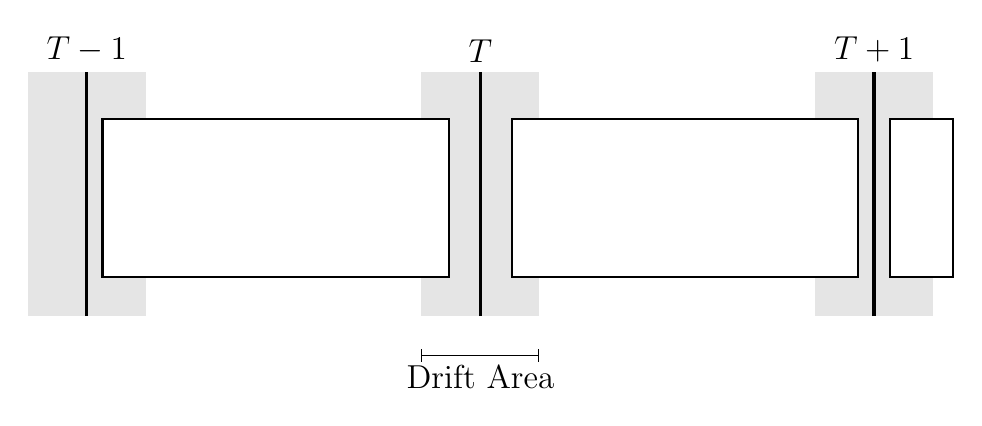
\begin{tikzpicture}[>=Latex, font=\large, scale=1, transform shape]
  \foreach \x in {0, 5, 10} {
    \fill[gray!20] (\x - 0.75, -1) rectangle (\x + 0.75, 2.1);
  }
  \draw[thick, fill=white] (0.2, -.5) rectangle (4.6, 1.5);
  \draw[thick, fill=white] (5.4, -.5) rectangle (9.8, 1.5);
  \draw[thick, fill=white] (10.2, -.5) rectangle (11.0, 1.5);
  \draw[|-|] (4.25, -1.5) -- (5.75, -1.5) node[midway, below] {Drift Area};
  
  \foreach \x/\label in {0/{$T-1$}, 5/{$T$}, 10/{$T+1$}} {
    \draw[very thick] (\x, -1) -- (\x, 2.1);
    \node[above, black] at (\x, 2.1) {\bfseries \label}; 
  }
\end{tikzpicture}
    \caption{Two objects whose $Size_{T_n} < Takt$. This is the most common case, as opposed to the more extreme cases shown in this thesis.}
\end{figure}

\begin{figure}[htbp]
\centering
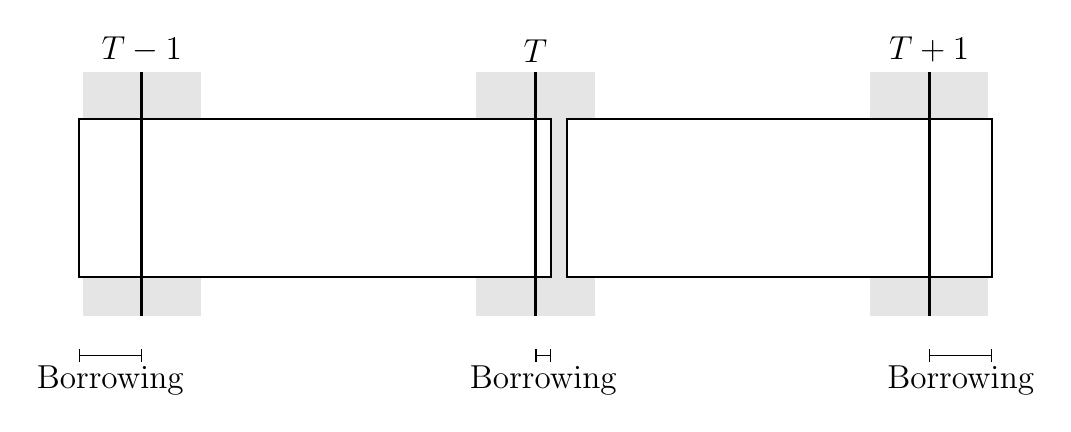
\begin{tikzpicture}[>=Latex, font=\large, scale=1, transform shape]
  \foreach \x in {0, 5, 10} {
    \fill[gray!20] (\x - 0.75, -1) rectangle (\x + 0.75, 2.1);
  }
  \draw[thick, fill=white] (-0.8, -.5) rectangle (5.2, 1.5);
  \draw[thick, fill=white] (5.4, -.5) rectangle (10.8, 1.5);
  \draw[|-|] (-.8, -1.5) -- (0, -1.5) node[midway, below] {Borrowing};
  \draw[|-|] (5, -1.5) -- (5.2, -1.5) node[midway, below] {Borrowing};
  \draw[|-|] (10, -1.5) -- (10.8, -1.5) node[midway, below] {Borrowing};
  
  \foreach \x/\label in {0/{$T-1$}, 5/{$T$}, 10/{$T+1$}} {
    \draw[very thick] (\x, -1) -- (\x, 2.1);
    \node[above, black] at (\x, 2.1) {\bfseries \label}; 
  }
\end{tikzpicture}
    \caption{Two objects whose $Size_{T_n} > Takt$. Both need to borrow time from their neighbouring stations in order to finish in time.}
\end{figure}
\section{Defining Overlaps}
\label{chap:overlap}

Overlaps stem from timing dependencies: each item’s "size" on a station $S_n$ depends on how long it takes for the item to process at the station. In other words, the "size" of the task is the duration of the task relative the duration of the station. If a task exceeds \textbf{Takt} in duration, then the use of the drift area is mandatory. 

However, if two items are processed consecutively at station $S_n$, and both of those items exceed \textbf{Takt} in $S_n$ to the point of requiring the usage of both of its neighbouring stations ($S_{n-1}$ and $S_{n+1}$), then there \textit{will} not be sufficient time for all operations to complete if both of those objects need to borrow time. These conflicting dependencies result in what's visualized as (and defined in this thesis as) an overlap, there simply isn't enough time for assembly to finish in time.

In practice the items do not literally stack or collide. Rather, the assembly line must halt in order to allow the operation to complete before the assembly line may continue again. 

Overlaps are how station overloads are visualized in this thesis, as we follow the constraint that no matter what, an allocation can never exceed $Takt + 2 * Drift$ in size, and an allocation can never go past the right-most limit of the drift area on the coming station.


\begin{figure}[htbp]
\centering

\begin{minipage}{0.45\textwidth}
\centering
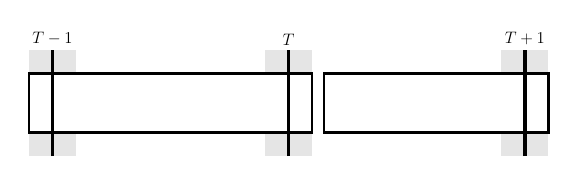
\begin{tikzpicture}[>=Latex, font=\large, scale=0.5, transform shape]

  \foreach \x in {0, 6, 2*6} {
    \fill[gray!20] (\x - 1.2/2, -0.6) rectangle (\x + 1.2/2, 1.5 + 0.6);
  }

  \draw[thick, fill=white] (-0.6, 0) rectangle (6 - 1.2/2+1.2, 1.5);
  
  \draw[thick, fill=white] (6 - 1.2/2+1.5, 0) rectangle (6*2 + 1.2/2, 1.5);

  \foreach \x/\label in {0/{$T-1$}, 6/{$T$}, 2*6/{$T+1$}} {
    \draw[very thick] (\x, -0.6) -- (\x, 1.5 + 0.6);
    \node[above, black] at (\x, 1.5 + 0.6) {\bfseries \label}; 
  }

\end{tikzpicture}
\caption{An example of two allocations, where there is enough room to borrow time for the larger one.}
\end{minipage}\hfill
\begin{minipage}{0.45\textwidth}
\centering
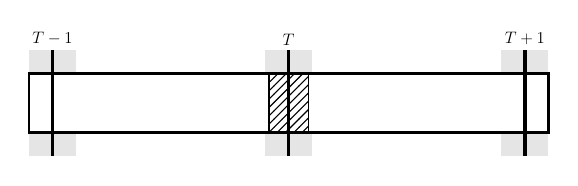
\begin{tikzpicture}[>=Latex, font=\large, scale=0.5, transform shape]

  \foreach \x in {0, 6, 2*6} {
    \fill[gray!20] (\x - 1.2/2, -0.6) rectangle (\x + 1.2/2, 1.5 + 0.6);
  }

  \draw[thick, fill=white] (-.6, 0) rectangle (6 + 0.5, 1.5);
  
  \draw[thick, fill=white] (6 - 0.5, 0) rectangle (2*6 + 1.2/2, 1.5);

  \draw[pattern=north east lines, pattern color=black] (6 - 0.5, 0) rectangle (6 + 0.5, 1.5);

  \foreach \x/\label in {0/{$T-1$}, 6/{$T$}, 2*6/{$T+1$}} {
    \draw[very thick] (\x, -0.6) -- (\x, 1.5 + 0.6);
    \node[above, black] at (\x, 1.5 + 0.6) {\bfseries \label};
  }

\end{tikzpicture}
\caption{An example of two allocations, where there is not enough room as both require borrowing, causing an overlap.}
\end{minipage}

\end{figure}

\chapter{State of the Art Analysis}
\label{ch:sota}


The Mixed-Model Assembly Line (MMAL) problem is an optimization problem, formally classified as NP-Hard. Traditionally, these optimization problems are addressed using heuristic or meta-heuristic algorithms, rather than using machine learning.

In recent years, Deep Reinforcement Learning (DRL) has become a dominant approach for solving dynamic scheduling problems. Unlike supervised methods, DRL agents learn through trial-and-error interaction with a simulation environment, aiming to maximize a cumulative reward signal. \cite{ref19} \cite{ref20}

For example, Chen et al. proposed an Adaptive Deep Q-Network, which builds on the Q-Learning Algorithm in order to address scheduling in Cloud Manufacturing environments characterized by stochastic task arrivals. Their approach utilizes a resizable network structure to adapt to changing machine availability and employs a complex reward mechanism to balance multiple objectives, such as minimizing work time, and optimizing machine load. \cite{ref10} 

However, reinforcement learning requires trying and failing repeatedly in order to learn, and applying such trial and error Reinforcement Learning methods to a Mixed-Model Assembly Line (MMAL), especially in a production environment, will pose significant risks. In a cloud environment, a scheduling error typically results in a slowdown in the form of increased latency or reduced throughput. In contrast, a scheduling error in a physical MMAL situation often results in scheduling overlaps that force the entire assembly line to halt in order for each station to be able to finish in time. Given these higher stakes, the exploratory nature of reinforcement learning agents may be prohibitively costly compared to imitating proven human strategies, hence the use of Deep Supervised Learning was chosen instead.

While DRL is effective for dynamic environments where rules change frequently, it presents significant implementation challenges. It requires the construction of a high-fidelity simulation environment and the careful engineering of state and action spaces. Furthermore, the "black box" nature of the reward signal makes it difficult to capture the nuanced, unwritten knowledge of the human servicemen, which is the primary objective of this thesis.

Current manual approaches rely heavily on the "tacit knowledge" of management staff, knowledge accumulated through experience that is difficult to articulate as explicit rules, especially if rules have accumulated over time. This thesis proposes capturing this knowledge using Supervised Learning,a paradigm formally known in this context as Imitation Learning. A precedent for this methodology is established by Dupuis et al. \cite{ref2}, who successfully trained a Sequence-to-Sequence (Seq2Seq) model using teacher-forcing to generate production schedules.


\section{Recurrent Architectures}
\label{sec:recurrent_arch}

To emulate the sequential decision-making process of human schedulers, we first investigate architectures adapted from Natural Language Processing (NLP) that process data sequentially.

\subsection{Long Short-Term Memory (LSTM)}
\label{subsec:lstm}

In previous works addressing similar scheduling problems, researchers have applied Recurrent Neural Networks (RNNs), often utilizing Long Short-Term Memory (LSTM) units within a sequence-to-sequence (Seq2Seq) framework \cite{ref2}.

A defining characteristic of LSTMs is their ability to selectively forget irrelevant or outdated information via the "forget gate". This mechanism allows the model to focus on relevant patterns over time, mitigating the vanishing gradient problem inherent in standard RNNs and improving the modeling of long-term dependencies \cite{ref4, ref9}.

\subsection{Sequence-to-Sequence (Seq2Seq) Models}

Seq2Seq models, typically built upon encoder-decoder RNN architectures, are designed to map an input sequence to an output sequence of a different length or order \cite{ref2}.  While traditionally applied to machine translation (e.g., transforming English to Swedish), this architecture is adaptable to the assembly line problem. In this context, the input is a sequence of vectorized product orders, and the output is the permuted production sequence \cite{ref3}.

However, applying standard Seq2Seq models to permutation problems presents a specific challenge: \textbf{vocabulary definition}. Standard NLP models select outputs from a fixed, pre-defined vocabulary, similar to a dictionary. In a manufacturing context, where every day's product list is unique, a fixed vocabulary is insufficient. The model must instead learn to select from the dynamic input available that day, a task that is non-trivial for standard Seq2Seq architectures unless they strictly rely on abstract sequence indices \cite{ref2, ref3}.

One way to remedy this limitation is to modify the decoder to point directly to the input elements, an approach that leads to the development of Pointer Networks,

\subsection{Limitations of Recurrent Architectures}

Despite their historical success, RNN and LSTM-based models suffer from a significant bottleneck: \textbf{sequential processing}. This is because these models must process the input sequence step-by-step, so that item $t$ depends on item $t-1$, they cannot parallelize computation either. This results in slower training times and, more importantly, a limited ability to capture a lot of global context across the entire schedule simultaneously \cite{ref4}.

This limitation motivates the shift toward \textbf{Attention-based approaches}, which process the entire sequence in parallel, and has a larger global context scope.

\section{Attention-Based Architectures}
\label{sec:attention_arch}

\subsection{The Transformer Model}
\label{subsec:transformer}

To address the sequential bottlenecks of RNNs, Transformer-based architectures discard recurrence entirely, relying instead on a self-attention mechanism \cite{ref5}.

The defining characteristic of the Transformer is the use of scaled dot-product attention. This allows the model to weigh the importance of each element in a given sequence relative to all other elements in that same sequence, regardless of distance. \cite{ref14} This parallelized computation not only accelerates training but enables the model to capture global dependencies more effectively than RNN-based methods. Since Transformers are order-agnostic, positional encodings are added to the input vectors to retain sequence order information \cite{ref5}.

For combinatorial scheduling problems, this translates into the ability to model complex interactions across the entire planning horizon. \cite{ref13} The placement of one item can be directly conditioned on all others in the same day's sequence, providing the context awareness necessary for effective assembly line scheduling \cite{ref8}.

\subsection{Pointer Networks}
\label{subsec:pointer_nets}

While Transformers excel at context, they still typically rely on generating tokens from a fixed vocabulary. The \textbf{Pointer Network} is the only architecture in this analysis specifically designed for combinatorial optimization and permutation problems \cite{ref7}.

Implemented using an encoder-decoder structure of the sequence-to-sequence model, the Pointer Network utilizes a specialized attention mechanism to generate context vectors that "point" to specific elements in the input sequence rather than predicting a value from a dictionary. 

This model is explicitly designed with combinatorial problems in mind, such as the traveling salesman problem, convex hull, and other combinatorial optimization problems. \cite{ref7} It is thus well-suited for the mixed-model assembly line problem (MMAL), as the object attributes (such as station order, or time to complete) are immutable, and the only thing that matters for our case is the permutation/rearrangement.


\chapter{Methodology}

\section {Data generation}
\subsection{Constants}
For data generation the following constants are used:
\begin{table}[htbp]
    \centering
    \caption{Table of Constants used in Data Generation}
    \label{tab:genconsts}
    \begin{tabular}{l c l} % Left-aligned, Centered, Left-aligned
        \toprule
        \textbf{Constant} & \textbf{Default Value} & \textbf{Description} \\ 
        \midrule
        Objects    & $100$     & Total number of objects in the testing sequence \\
        Stations   & $39$      & Number of stations \\
        Takt       & $700$     & The cycle time ($Cmin$) \\
        Drift      & $200$     & The size of the drift area ($Cmin$) \\
        Gap        & $10$      & Time-buffer ($Cmin$) between generated objects \\
        min\_size  & $100$     & Smallest possible Object ($Cmin$) \\
        max\_size  & $Takt + 2 \times Drift$ & Largest possible Object ($Cmin$) \\
        Multiplier & $5000$    & Constant value to multiply \textit{Objects} with, used for Training.\\
        \bottomrule
    \end{tabular}
\end{table}
\subsection{Data Preprocessing and Abstraction}
For the purpose of training optimization, the raw information is abstracted into a concise JSON schema. Each entry in the dataset is reduced to the following three attributes:

\begin{itemize}
    \item \textbf{Object ID} (\texttt{object}): An integer representing the unique identifier of the item.
    \item \textbf{Station Data} (\texttt{data}): A mapping of station keys ($s_1, \dots, s_{35}$) to their respective time requirement values.
    \item \textbf{Station Offsets} (\texttt{offsets}): A mapping of station keys to their relative offset values.
\end{itemize}

By utilizing these values, we can train a model to prioritize time-based decision-making over rigid rule-based systems. It is important to note that while the model operates without explicit constraints, the use of a sufficiently large dataset derived from expert tacit knowledge ensures that it implicitly adheres to fundamental ground rules, albeit with greater flexibility.

\subsection{Offset Calculation and Centering}
The positioning of an object within a station is determined by its \textit{offset} relative to the \textbf{Takt} start ($0$ locally). The script employs a dynamic centering logic that positions tasks within the remaining available capacity of the standard Takt window. This approach balances the empty space (or buffer) on either side of the allocation, adapting to the finish time of the preceding task.

To determine the position, the script first calculates the local start time, $t_{start}$, which corresponds to the completion of the previous allocation relative to the current Takt. The remaining buffer, $B$, is calculated as the difference between the standard Takt duration $T$ and the occupied time, clamped to zero to ensure non-negative spacing:

\begin{equation}
    B = \max(0, T - t_{start} - S)
\end{equation}

Where $S$ is the size (duration) of the new task. The tentative offset, $O_{calc}$, is then derived by placing the task at the start position plus half of the calculated buffer:

\begin{equation}
    O_{calc} = t_{start} + \frac{B}{2}
\end{equation}

This formula ensures that if the previous task finishes early, the new task is centered in the wide gap; if the previous task finishes late, the buffer shrinks, effectively pulling the new task closer to the previous one.

Finally, to ensure the object adheres to physical station boundaries and drift limitations ($D$), the calculated offset is clamped. The maximum permissible offset is defined such that the task end does not exceed the drift limit ($T+D$):

\begin{equation}
    O_{calc} = \max(-D, \min(O_{calc}, T + D - S))
    \label{eq:offset_constraint}
\end{equation}

\begin{figure}[htbp]
\centering

\begin{minipage}{0.48\textwidth}
\centering
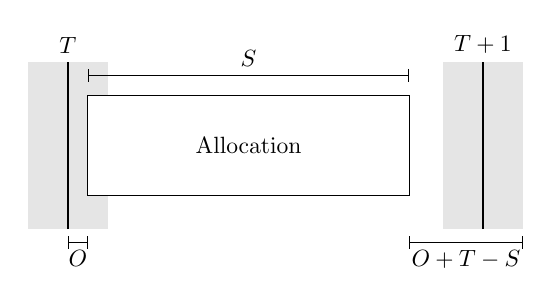
\begin{tikzpicture}[>=Latex, scale=0.85, transform shape]

  \fill[gray!20] (-1.2, -0.5) rectangle (0, 2);

  \fill[gray!20] (5, -0.5) rectangle (6.2, 2);

  \draw[draw, fill=white] (-0.3,0) rectangle (4.5, 1.5) node[pos=.5] {Allocation};

  \draw[thick] (-0.6, -0.5) -- (-0.6, 2);
  \draw[thick] (5.6, -0.5) -- (5.6, 2);

  \node[above] at (-0.6, 2) {$T$};
  \node[above] at (5.6, 2) {$T+1$};

  \draw[|-|] (-0.3, 1.8) -- (4.5, 1.8) node[midway, above] {$S$};

  \draw[|-|] (-0.6, -0.7) -- (-0.3, -0.7) node[midway, below] {$O$};

  \draw[|-|] (4.5, -0.7) -- (6.2, -0.7) node[midway, below] {$O + T - S$};

\end{tikzpicture}
    \caption{Allocation positioning before the centering process}
\end{minipage}\hfill
\begin{minipage}{0.48\textwidth}
\centering
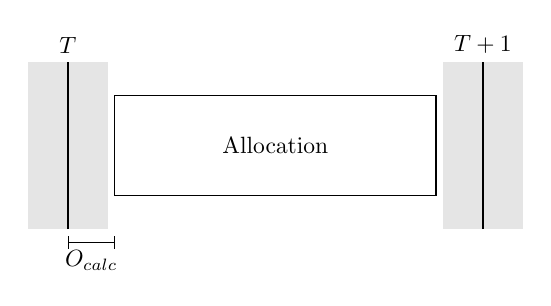
\begin{tikzpicture}[>=Latex, scale=0.85, transform shape]

  \fill[gray!20] (-1.2, -0.5) rectangle (0, 2);

  \fill[gray!20] (5, -0.5) rectangle (6.2, 2);

  \draw[draw, fill=white] (0.1,0) rectangle (4.9, 1.5) node[pos=.5] {Allocation};

  \draw[thick] (-0.6, -0.5) -- (-0.6, 2);
  \draw[thick] (5.6, -0.5) -- (5.6, 2);

  \node[above] at (-0.6, 2) {$T$};
  \node[above] at (5.6, 2) {$T+1$};

  \draw[|-|] (-0.6, -0.7) -- (0.1, -0.7) node[midway, below] {$O_{calc}$};

\end{tikzpicture}
\caption{Allocation after centering.}
\end{minipage}

\end{figure}

\subsection{Constructive Data Generation as a Solved Puzzle} 
\label{sub:datagen}

To train the machine learning model, a synthetic dataset is required that represents valid, collision-free production schedules. Rather than placing tasks stochastically and checking for validity, the system employs a constructive generation algorithm which builds one object at the time. This approach acts as a forward simulation, placing allocations sequentially to inherently create a "solved puzzle" which serves as the ground truth for training. Due to how the entire sequence generates left to right the risk for overlaps is nonexistent.

\subsubsection*{Dependency-Based Positioning}
The placement of any given allocation $A_{[T_n , S_n]}$ (Timeslot $T_n$ at Station $S_n$) is not independent. It is strictly constrained by two spatial-temporal boundaries derived from the existing grid state:
\begin{enumerate}
    \item \textbf{Station Availability:} The station $S_n$ must be free. Therefore, $A_{[T_n , S_n]}$ cannot start until the previous object at $T_{n-1}$ has departed station $S_n$.
    \item \textbf{Object Availability:} The object at $T_n$ must be ready. Therefore, $A_{[T_n , S_n]}$ cannot start until the object at $T_n$ has finished processing at the previous station $S_{n-1}$.
    \item \textbf{Gap (Density control):} To vary the complexity of the generated data, a gap is introduced (see \ref{tab:genconsts}). A larger gap will result in sparser schedules with multiple valid solutions, whereas a minimal gap will result in densely packed schedules. In a real-world manufacturing context, tighter schedules would maximize throughput but place higher strain on human operators.
\end{enumerate}

Mathematically, the earliest valid start time ($t_{start}$) for the new allocation is defined as the maximum of these two completion timestamps, plus a configured safety gap:

\begin{equation}
    t_{start} = \max(End_{T_{n-1}, S_n}, \quad End_{T, S_{n-1}}) + Gap
\end{equation}

This logic ensures that the generated schedule is causally valid, no object effectively "teleports" between stations, and no two objects overlap on a single station.

\subsubsection*{Context-Aware Scaling}
The dimensions of the tasks are also generated dependently. While duration in each station for each object is chosen stochastically, the actual assigned size ($S$) of the duration is clamped by the remaining available time in the Takt + Drift window. The generator calculates the available space between the calculated $t_{start}$ and the maximum drift boundary. If the random size exceeds this space, it is truncated to fit (within the constraints of $min\_size$, see \ref{tab:genconsts})

\begin{equation}
    min\_size \leq S \leq max\_size 
    \label{eq:}
\end{equation}

Wehen training the model is fed the sorted list, while testing is fed never seen before shuffled data. This process results in a synthetic dataset where every input sequence has a perfectly matching output sequence that is guaranteed to be solvable, providing a robust target for supervised learning.

\begin{figure}[H] 
\centering
\begin{minipage}{0.48\textwidth}
    \centering
    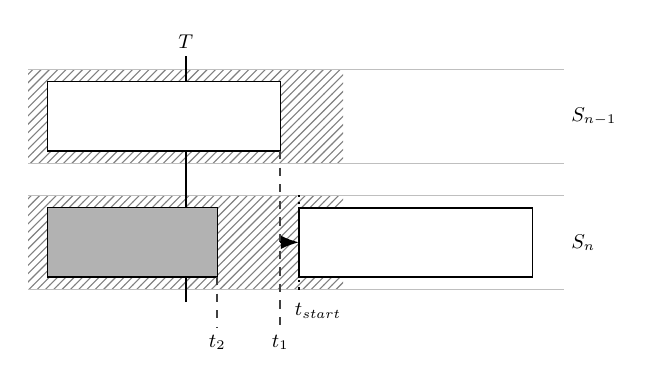
\begin{tikzpicture}[>=Latex, font=\small, scale=0.8, transform shape]

        \fill[pattern=north east lines, pattern color=gray] (-2.5, 2.0) rectangle (2.5, 3.5);
        \fill[pattern=north east lines, pattern color=gray] (-2.5, 0) rectangle (2.5, 1.5);
        \draw[gray!50] (-2.5, 2.0) -- (6, 2.0);
        \draw[gray!50] (-2.5, 3.5) -- (6, 3.5);
          
        \draw[gray!50] (-2.5, 0) -- (6, 0);
        \draw[gray!50] (-2.5, 1.5) -- (6, 1.5);

        % Added Station Labels
        \node[right] at (6, 2.75) {$S_{n-1}$};
        \node[right] at (6, 0.75) {$S_{n}$};

        \draw[thick] (0, -0.2) -- (0, 3.7);
        \node[above] at (0, 3.7) {$T$};
        \draw[fill=white, draw=black] (-2.2, 2.2) rectangle (1.5, 3.3);

        \draw[thick, dashed, darkgray] (1.5, 2.2) -- (1.5, -0.6);
        \node[below] at (1.5, -0.6) {$t_{1}$};

        \draw[fill=gray!60, draw=black] (-2.2, 0.2) rectangle (0.5, 1.3);

        \draw[thick, dashed, darkgray] (0.5, 0.2) -- (0.5, -0.6);
        \node[below] at (0.5, -0.6) {$t_{2}$};
         
        \draw[fill=white, draw=black, thick] (1.8, 0.2) rectangle (5.5, 1.3);
        \fill[white] (5.2, 0.22) rectangle (5.5, 1.28);
         
        \node[font=\bfseries] at (3.65, 0.75) {};

        \draw[->, thick, black] (1.5, 0.75) -- (1.8, 0.75);
        \draw[dotted, thick] (1.8, 0) -- (1.8, 1.5);
        \node[below] at (2.1, -0.1) {$t_{start}$};

    \end{tikzpicture}
    \caption{Case 1: The white object in $S_{n-1}$ is borrowing time from itself at $S_n$, and thus cannot begin assembly at $S_n$ until it has finished the task at $S_{n-1}$.}
\end{minipage}\hfill
\begin{minipage}{0.48\textwidth}
    \centering
    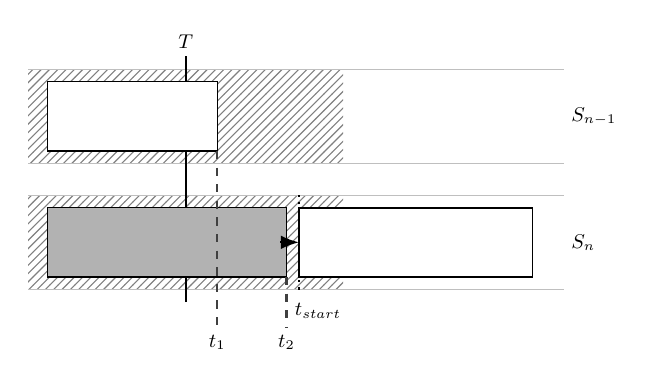
\begin{tikzpicture}[>=Latex, font=\small, scale=0.8, transform shape]

        \fill[pattern=north east lines, pattern color=gray] (-2.5, 2.0) rectangle (2.5, 3.5);
        \fill[pattern=north east lines, pattern color=gray] (-2.5, 0) rectangle (2.5, 1.5);
        \draw[gray!50] (-2.5, 2.0) -- (6, 2.0);
        \draw[gray!50] (-2.5, 3.5) -- (6, 3.5);
          
        \draw[gray!50] (-2.5, 0) -- (6, 0);
        \draw[gray!50] (-2.5, 1.5) -- (6, 1.5);

        % Added Station Labels
        \node[right] at (6, 2.75) {$S_{n-1}$};
        \node[right] at (6, 0.75) {$S_{n}$};

        \draw[thick] (0, -0.2) -- (0, 3.7);
        \node[above] at (0, 3.7) {$T$};
        \draw[fill=white, draw=black] (-2.2, 2.2) rectangle (0.5, 3.3);


        \draw[fill=gray!60, draw=black] (-2.2, 0.2) rectangle (1.6, 1.3);
          
        \draw[fill=white, draw=black, thick] (1.8, 0.2) rectangle (5.5, 1.3);
        \fill[white] (5.2, 0.22) rectangle (5.5, 1.28);
          
        \node[font=\bfseries] at (3.65, 0.75) {};

        \draw[thick, dashed, darkgray] (.5, 2.2) -- (.5, -0.6);
        \node[below] at (.5, -0.6) {$t_{1}$};

        \draw[thick, dashed, darkgray] (1.6, 0.2) -- (1.6, -0.6);
        \node[below] at (1.6, -0.6) {$t_{2}$};

        \draw[->, thick, black] (1.5, 0.75) -- (1.8, 0.75);
        \draw[dotted, thick] (1.8, 0) -- (1.8, 1.5);
        \node[below] at (2.1, -0.1) {$t_{start}$};

    \end{tikzpicture}
    \caption{Case 2: The gray object is borrowing time from the white object in $S_n$. Even though it finished in $S_{n-1}$, the white object cannot begin assembly right away in $S_n$ as it's dependent on the gray object finishing at $S_n$.}
\end{minipage}
\end{figure}

\section{Adapting Language-Based Models for Sequencing}

Two of the models examined in this thesis, the Sequence-To-Sequence model and the Transformer model, were originally designed for natural language processing (NLP) tasks. These models typically rely on a fixed, predefined vocabulary.

This reliance proves problematic because the processed data in this thesis does not consist of static words from a dictionary, rather a dynamic set of \textit{unique} objects that changes with every production batch. Consequently, the model cannot predict a token from a learned list, rather it must instead select from the variable input provided on that sequence.

Furthermore, specific combinatorial constraints must be imposed. Natural language generation is probabilistic and inherently allows for repetition, and if poorly trained might default to the "easiest" alternative. (e.g., the word "the" repeating multiple times, due to it being the most common word in the english language). 

In our use-case, each object within the input \textit{must} appear in the output sequence \textit{exactly once}, and the length of the output sequence \textit{must} match the length of the input sequence. Therefore, the architecture must be adapted to enforce this combinatorial constraint, ensuring valid permutations rather than simply generating the most statistically probable tokens (see \ref{chap:workarounds}).

\section{Workarounds}
\label{chap:workarounds}

The Transformer and Sequence-To-Sequence models have been adapted from their original NLP architectures to a permutation architecture in order to address combinatorial problems. The Pointer Network remains unaffected by these modifications.

\subsection{Direct Continuous Input}

The Sequence-To-Sequence model is implemented here without an Embedding layer. Instead of projecting vocabulary indices into a latent embedding space, this module is omitted to allow raw feature vectors to be processed directly. This enables the model to interpret the specific magnitudes and geometric properties of input elements as continuous values rather than abstract symbols. This approach is particularly well-suited for combinatorial tasks, as it preserves intrinsic numerical relationships in the data that would otherwise be obscured by tokenization.

\subsection{Soft Decoding}

The Sequence-To-Sequence model employs a "soft" feedback loop during sequence generation. In traditional language processing, the decoder typically commits to a single discrete choice by selecting the most probable word and treating it as the ground truth for the subsequent step. In this context, however, rigid early choices can trap the model in sub-optimal paths. To mitigate this, the model feeds the full probability distribution into the next step rather than a single discrete selection. By propagating uncertainty rather than discarding it, the system can dynamically refine its strategy as the output sequence is constructed.

\subsection{The Pointer Head}
\label{sub:phead}

The greatest deviation from the canonical Transformer is the removal of the vocabulary projection layer. It is replaced by a \texttt{PointerHead} module designed to select elements from the input sequence, a mechanism inspired by the Pointer Network \ref{sec:pointer}.

Instead of predicting a token from a fixed vocabulary, the Pointer Head computes a similarity score between the current decoder state and the encoder outputs using the Transformer's attention mechanism, rather than additive attention \cite{ref5} \cite{ref7}:
 \begin{equation}
    \text{Scores} = \frac{(Dec_{out} W_q) \cdot (Enc_{out} W_k)^T}{\sqrt{d_{model}}}
\end{equation} 
These raw logit scores represent the compatibility between the current decoding step and every element in the input sequence. When passed through a Cross-Entropy loss function during training, they effectively train the model to "point" to the correct input index for the next position in the sequence.

\chapter{System Architecture}

\section{Machine Learning Models}

The models in this thesis are implemented using PyTorch.

\begin{table}[htbp]
    \centering
    \caption{Hyperparameters and Model Constants}
    \label{tab:generation_constants}
    \begin{tabular}{l c c c} 
        \toprule
        \textbf{Constant} & \textbf{Transformer} & \textbf{Sequence-To-Sequence} & \textbf{Pointer Network} \\ 
        \midrule
        batch\_size & $16$ & $16$ & $8$ \\
        num\_epochs & $10$ & $10$ & $10$ \\
        lr & $1e^{-3}$ & $1e^{-4}$ & $1e^{-4}$ \\
        d\_model & $256$ & $256$ & $256$ \\
        dropout & $0.1$ & $0.2$ & $ $ \\
        hidden\_dim & $ $ & $128$ & $128$ \\
        d\_ff & $512$ & $ $ & $ $ \\
        n\_heads & $8$ & $ $ & $ $ \\
        n\_layers & $3$ & $ $ & $ $ \\
        \bottomrule
    \end{tabular}
\end{table}




\subsection{The Transformer Model}
\label{sec:trans}
The implemented model adapts the standard Transformer architecture originally proposed by Vaswani et al. \cite{ref5} to handle continuous combinatorial data. Unlike standard NLP models that process discrete tokens, this implementation operates on continuous feature vectors and utilizes a pointer mechanism for output generation.

\subsubsection{Continuous Input Embeddings}
Standard Transformers typically utilize a lookup table to map discrete vocabulary indices to dense vectors. Since the input data for this problem consists of continuous immutable features (station order (always 1 - n), station times, dimensions), the embedding layer is replaced by a learnable linear projection. 

\subsubsection{Positional Encoding}
As the Transformer architecture contains no recurrence or convolution, it can thus not distinguish the order of the input objects, essentially treating it as an unordered set. To address this, a fixed sinusoidal Positional Encoding is added to the input embeddings. This provides each element with a unique geometric signature, allowing the model to determine the relative positions of objects within the sequence. The encodings are calculated as \cite{ref5}:
\begin{equation}
    PE_{(pos, 2i)} = \sin(pos / 10000^{2i/d_{model}})
\end{equation}
\begin{equation}
    PE_{(pos, 2i+1)} = \cos(pos / 10000^{2i/d_{model}})
\end{equation}
This mechanism allows the model to distinguish between identical tasks placed at different positions in the sequence.

\subsubsection{Layer Normalization and Pre-Norm Formulation}
The system employs Layer Normalization to stabilize training \cite{ref1}, specifically adopting "Pre-Normalization" where the input is normalized \textit{before} passing it to the sub-layer, rather than after. This configuration, implemented in the \texttt{ResidualConnection} module, allows gradients to flow more directly through the network, generally improving convergence in deeper models.

\subsubsection{Multi-Head Attention}
The core mechanism of the model is Multi-Head Attention (MHA), which allows the model to jointly attend to information from different representation subspaces. The implementation utilizes $h$ parallel heads. For each head, the input is projected into Query, Key, and Value ($Q$, $K$, $V$) matrices. The attention scores are computed using Scaled Dot-Product Attention: \cite{ref5}
\begin{equation}
    \text{Attention}(Q, K, V) = \text{softmax}\left(\frac{QK^T}{\sqrt{d_k}}\right)V
\end{equation}

\subsubsection{Feed-Forward Block}
Each encoder and decoder layer contains a position-wise Feed-Forward Network (FFN). This consists of two linear transformations with a ReLU activation function in between: \cite{ref5}
\begin{equation}
    FFN(x) = \text{ReLU}(xW_1 + b_1)W_2 + b_2
\end{equation}
The inner layer projects the input to a higher dimension ($d_{ff}$, typically $4 \times d_{model}$) before projecting it back, introducing additional non-linearity to the model.

\subsubsection{The Pointer Head}

This implementation of the Transformer replaces the vocabulary projection layers in favour of a Pointer Head in order to handle combinatorial tasks rather than NLP-based tasks. See \ref{sub:phead}

\subsection{Sequence-to-Sequence}
\label{sec:seq2seq}

The implemented model is a standard Sequence-To-Sequence model with modifications clarified in \ref{chap:workarounds}.

\subsubsection{Continuous Input Encoder}
The \texttt{EncoderRNN} processes the input sequence to generate a latent representation of the problem state. Unlike standard NLP encoders that require an embedding layer to project discrete tokens, this module accepts raw feature vectors directly. 

\subsubsection{Attention Mechanism}
To overcome the bottleneck of compressing the entire sequence into a single fixed-length vector, the model employs an Attention mechanism, referred to as Bahdanau Attention \cite{ref16}. This approach allows the decoder to "search" the entire input sequence and dynamically focus only on the information relevant to the current step.

Rather than relying on a static summary of the input, the mechanism calculates a dynamic "relevance score" for every item in the input sequence. These scores effectively function as a spotlight, determining how much focus the model should place on each specific input element when generating the next part of the output.

These scores are normalized into probabilities that sum to 100\%. Finally, the model computes a time dependent Context Vector ($c_t$), which is a weighted average of the inputs \cite{ref16}:
\begin{equation}
    c_t = \sum_{j=1}^{T_x} \alpha_{tj} h_j
\end{equation}
This weighted sum ensures that the model prioritizes the most relevant information for the immediate prediction while ignoring irrelevant noise, effectively bypassing the long-term memory limitations of standard Recurrent Neural Networks.

\subsubsection{Context-Aware Decoder}
The decoder (\texttt{DecoderRNN}) generates the output sequence step-by-step. To maximize the utility of the attention mechanism, the context vector $c_t$ is injected at two distinct points in the decoding step:
\begin{enumerate}
    \item \textbf{Input Feeding:} The context vector is concatenated with the input of the current time step before being passed to the LSTM.
    \item \textbf{Output Projection:} The context vector is concatenated with the LSTM output before the final linear projection layer.
\end{enumerate}
This structure ensures that both the recurrent processing and the final prediction are directly conditioned on the relevant parts of the source input.


\subsection{The Pointer Network Model}
\label{sec:pointer}

The proposed solution implements a Pointer Network architecture adapted from Vinyals et al. (2015). \cite{ref7} The model follows an Encoder/Decoder paradigm enhanced with an attention mechanism, specifically designed to handle variable-length input sequences and output a permutation of the input indices.

\subsubsection{Encoder Mechanism}
The encoder processes the input sequence to generate a latent representation of the problem state.
\begin{enumerate}
    \item \textbf{Input Projection:} Raw input features are first passed through a \texttt{Projector} block. This module consists of a Linear Transformation, an Tanh Activation, and Layer Normalization. \cite{ref1}
    \item \textbf{Bidirectional LSTM:} The projected features are fed into a bidirectional LSTM. This allows the model to capture context from both past and future states in the sequence. 
\end{enumerate}

\subsubsection{Decoder and Attention Mechanism}
The decoder generates the output permutation one index at a time. Unlike standard NLP models that generate new tokens from a fixed vocabulary, this decoder selects indices directly from the input sequence.

\begin{itemize}
    \item \textbf{Glimpse Mechanism:} To enhance the pointing accuracy, the model employs a "glimpse" mechanism as proposed by Vinyals et al. (2016) \cite{ref18}. Unlike the standard Pointer Network which points immediately, this mechanism allows the decoder to "reason" about the global context before making a selection. At time step $t$, the decoder state $s_t$ queries the encoder outputs to calculate a context vector $c_t$ \cite{ref18}:
    \begin{equation}
        c_t = \sum_{i=1}^{T} \text{Attention}(s_t, h_i) \cdot h_i
    \end{equation}
    This vector summarizes the most relevant parts of the input sequence for the current decision.

    \item \textbf{Pointer Selection:} The final selection is performed by fusing the glimpse context with the original state. The context vector $c_t$ is projected and added to the current decoder state (a residual connection) to form a \textit{refined query} $u_t$:
    \begin{equation}
        u_t = s_t + \tanh(W_{proj} \cdot c_t)
    \end{equation}
    This refined query $u_t$ is then used to compute the final attention scores (logits) over the input elements. The index with the highest probability is selected as the next element in the permutation.
\end{itemize}

\subsubsection{Masking and Inference}
To ensure the validity of the resulting permutation (i.e., the Traveling Salesman constraint that every city is visited exactly once), a masking mechanism is applied during inference. 

Once an input index $k$ is selected, it is masked out by setting its log-probability to $-\infty$ ($1e^{-9}$) for all subsequent steps. This hard constraint prevents the model from selecting the same element twice. Furthermore, the model is auto-regressive: the feature vector of the selected element $h_k$ is used as the input to the decoder for the next time step $t+1$.

\clearpage
\section{The Dataset}
To train the models, a custom PyTorch Dataset was implemented to handle combinatorial data. This pipeline is responsible for converting raw input jsons into tensors. The dataset looks more or less the same for all models.

\subsection{Data Processing}
The dataset is initialized with raw JSON files containing sequences of station data. The pipeline flattens these structures into a stack of tensors, where each tensor represents a single task sequence with the shape:

\begin{equation}
    X = \begin{bmatrix}
    x_{1,1} & x_{1,2} & \dots & x_{1,N} \\
    x_{2,1} & x_{2,2} & \dots & x_{2,N} \\
    \vdots & \vdots & \ddots & \vdots \\
    x_{M,1} & x_{M,2} & \dots & x_{L,N}
    \end{bmatrix}
\end{equation}

Where $N$ is the number of stations and $M$ is the the number of objects. 

The feature extraction is performed by selecting specific keys ($s_1 \dots s_N$) from the raw data objects. To ensure numerical stability and faster converges the data is then normalized using: 
\begin{equation}
    x_{norm} = \frac{x_{raw}}{1000.0}
\end{equation}
Due to memory constraints, the sequences exceeding the maximum defined length are chunked into smaller subsequences to manage memory constraints effectively.

\subsection{Shuffled Task Generation}
 The dataset stores the ground truth sequences in their correct, sorted order. However, the data is effectively augmented during the training phase by randomly shuffling the input sequence at every iteration. This stochastic approach ensures that the model encounters the same sequence twice.

To accommodate this shuffling, the target vector is dynamically generated to represent the specific indices required to reconstruct the original order from the disordered input. If the shuffled input is denoted as $X'$ and the original sorted sequence as $X$, the target index $y_t$ for time step $t$ is calculated to satisfy the condition:
\begin{equation}
    X'[y_t] = X_t
\end{equation}
This formulation specifically trains the Pointer Mechanism of the Transformer and Pointer Network to identify the location of the next correct element within the provided input set. (And then "point" to it)

\section{The Training Loop}
\label{sec:training}

To ensure a fair and consistent evaluation, a standardized training pipeline is implemented across all three architectures (Seq2Seq, Pointer Network, and Transformer). The training logic is built using the PyTorch framework and orchestrates data loading, gradient optimization, and model persistence.

\subsection{Optimization and Objective Function}
Model parameters are optimized using the \textbf{AdamW} algorithm \cite{ref15}. This optimizer was selected for its ability to decouple weight decay from adaptive gradient updates, a modification that consistently yields better generalization than the standard Adam implementation. The learning rate is set to $1 \times 10^{-4}$ and the weight decay is set to $1 \times 10^{-2}$.

The model is trained to minimize the \textbf{Cross-Entropy Loss} between the output logits and the target sequence. A masking constraint (\texttt{ignore\_index=-1}) is applied to handle variable sequence lengths within batches. This effectively isolates the padding tokens from the objective function, ensuring the optimization focuses solely on valid data elements rather than padding.

\subsection{Regularization and Stabilization}
Training deep neural networks, particularly those involving recurrence (RNNs), can be unstable due to the exploding gradient problem. \cite{ref17} To mitigate this, Gradient Clipping is applied to the model parameters. This acts as a safety mechanism that caps the maximum possible step size during backpropagation. By preventing drastic weight updates, it ensures that outliers in the training data or instabilities in the recurrent layers do not cause the optimization process to diverge.

\subsection{Transformer Specifics: Masking strategy}
Unlike the recurrent models, which process data sequentially by definition, the Transformer processes the entire sequence in parallel. To replicate the sequential nature of the problem and prevent information leakage, a dual-masking strategy is implemented within the training loop via the \texttt{make\_masks} function:

\begin{enumerate}
    \item \textbf{Padding Mask (Source):} This mask identifies padding tokens in the input batch. It forces the self-attention mechanism to assign zero attention weights to these positions, ensuring the model focuses only on valid tasks.
    \item \textbf{Look-Ahead Mask (Target):} To preserve the auto-regressive property, a triangular "no-peak" mask is applied to the decoder. This ensures that when generating the prediction for position $t$, the model can only attend to positions $0$ through $t-1$, effectively hiding future ground-truth tokens.
\end{enumerate}

\subsection{Teacher Forcing}
\label{sec:teacher_forcing}

The method of training used in this thesis is refered to as "Teacher Forcing". The model is trained by supplying the ground-truth tokens from the previous time step ($t-1$) as input to predict the current time step ($t$), rather than feeding back the model's own generated prediction. This stabilizes training and enables faster convergence, especially in RNN-based models. \cite{ref2, ref21}

We apply this strategy across all three architectures, though the implementation differs due to the nature of the models:

\begin{enumerate}
    \item \textbf{Recurrent Models (Seq2Seq \& Pointer Network):} For the RNN-based architectures, Teacher Forcing is applied sequentially. During the forward pass, the decoder receives the ground-truth token $y_{t-1}$ explicitly at each time step to compute the hidden state and output for time $t$. \cite{ref2}
    \item \textbf{Transformer:} As the Transformer processes sequences in parallel, Teacher Forcing is implemented implicitly via the \textbf{Look-Ahead Mask} described previously. By masking future positions, the self-attention mechanism at position $t$ is restricted to attending only to the ground-truth sequence indices $[0, t-1]$, effectively replicating the Teacher Forcing behavior without a recurrent loop. \cite{ref22} \cite{ref5}
\end{enumerate}


\section{The Application Programming Interface (API)}
The system exposes its core functionalities through a RESTful API, facilitating programmatic interaction with the implemented neural architectures. This interface serves as the primary gateway for data ingestion and inference execution.

\subsection{Endpoints}

\subsubsection{/run/\{model\_type\}}

This POST endpoint provides a unified interface for sequence processing across different model architectures (\textbf{Transformer}, \textbf{Pointer Network}, or \textbf{Seq2Seq}). Once selected it returns a processed sequence made from the input data, including refitting. 

\subsubsection{/run/\{model\_type\}/$int:n$/}

This POST endpoint extends the interface to support multiple sequence generation. It accepts an integer parameter $n$, executing the selected model architecture $n$ times to return a list of $n$ alternative processed sequences.

\subsubsection{/check/}

This POST endpoint will count the number of \textbf{overlaps} on a given sequence, based on configuration data.

% INSERT?

\chapter{Experiments and results}
\section{Task Performance}
Performance is measured by how well the model can take an input with overlapping data and rearrange the tasks to minimize overlaps. The reduction metric is defined at \ref{sec:eval}.

Although the operational constraints of the target problem typically limit sequences to batches of roughly 100 objects, the following results also evaluate the model's scalability beyond this range.

The values in the tables below is based on the ratio found at \ref{sec:eval} $\frac{O_P}{O_S}$, where $O_S$ is the number of overlaps found in a freshly generated shuffled dataset, and $O_P$ is the number of overlaps found after predicting and processing the items in said dataset. With the improvement rate being defined as 
\begin{equation}
    Improvement = ( 1 - \frac{O_P}{O_S} ) \cdot 100 \%
\end{equation}

he testing data has an optimal solution before getting shuffled where $O_P = 0$. The data is generated using a random number generator, using no seed, to ensure variability across test runs.

\subsection{Pointer Network Performance}

\begin{table}[H]
    \centering
    \small 

    \begin{minipage}[t]{0.48\textwidth}
        \centering
        \caption{Test-size of $10$}
        \label{tab:res_10}
        \begin{tabular}{l c c}
            \toprule
            \textbf{Run} & \textbf{Ratio ($R$)} & \textbf{Red.} \\
            \midrule
            Run \#1 & $14/72$ & $80.56\%$ \\
            Run \#2 & $15/68$ & $77.94\%$ \\
            Run \#3 & $21/67$ & $68.66\%$ \\
            \midrule
            \textbf{Avg} & & $75.72\%$ \\
            \bottomrule
        \end{tabular}
    \end{minipage}
    \hfill
    \begin{minipage}[t]{0.48\textwidth}
        \centering
        \caption{Test-size of $100$}
        \label{tab:res_100}
        \begin{tabular}{l c c}
            \toprule
            \textbf{Run} & \textbf{Ratio ($R$)} & \textbf{Red.} \\
            \midrule
            Run \#1 & $188/713$ & $73.63\%$ \\
            Run \#2 & $183/741$ & $75.30\%$ \\
            Run \#3 & $180/719$ & $74.97\%$ \\
            \midrule
            \textbf{Avg} & & $74.63\%$ \\
            \bottomrule
        \end{tabular}
    \end{minipage}

    \vspace{0.8cm} 

    \begin{minipage}[t]{0.48\textwidth}
        \centering
        \caption{Test-size of $1000$}
        \label{tab:res_100b}
        \begin{tabular}{l c c}
            \toprule
            \textbf{Run} & \textbf{Ratio ($R$)} & \textbf{Red.} \\
            \midrule
            Run \#1 & $2008/7208$ & $72.14\%$ \\
            Run \#2 & $2013/7234$ & $72.17\%$ \\
            Run \#3 & $2031/7266$ & $72.05\%$ \\
            \midrule
            \textbf{Avg} & & $72.12\%$ \\
            \bottomrule
        \end{tabular}
    \end{minipage}
    \hfill
    \begin{minipage}[t]{0.48\textwidth}
        \centering
        \caption{Test-size of $10000$}
        \label{tab:res_100c}
        \begin{tabular}{l c c}
            \toprule
            \textbf{Run} & \textbf{Ratio ($R$)} & \textbf{Red.} \\
            \midrule
            Run \#1 & $20329/72702$ & $72.04\%$ \\
            Run \#2 & $20001/72463$ & $72.40\%$ \\
            Run \#3 & $20151/72567$ & $72.23\%$ \\
            \midrule
            \textbf{Avg} & & $72.22\%$ \\
            \bottomrule
        \end{tabular}
    \end{minipage}
\end{table}


\subsection{Transformer Performance}

\begin{table}[H]
    \centering
    \small 

    \begin{minipage}[t]{0.48\textwidth}
        \centering
        \caption{Test-size of $10$}
        \label{tab:res_10}
        \begin{tabular}{l c c}
            \toprule
            \textbf{Run} & \textbf{Ratio ($R$)} & \textbf{Red.} \\
            \midrule
            Run \#1 & $7/80$ & $91.25\%$ \\
            Run \#2 & $4/58$ & $93.10\%$ \\
            Run \#3 & $8/64$ & $87.50\%$ \\
            \midrule
            \textbf{Avg} & & $90.62\%$ \\
            \bottomrule
        \end{tabular}
    \end{minipage}
    \hfill
    \begin{minipage}[t]{0.48\textwidth}
        \centering
        \caption{Test-size of $100$}
        \label{tab:res_100}
        \begin{tabular}{l c c}
            \toprule
            \textbf{Run} & \textbf{Ratio ($R$)} & \textbf{Red.} \\
            \midrule
            Run \#1 & $73/721$ & $89.88\%$ \\
            Run \#2 & $76/734$ & $89.85\%$ \\
            Run \#3 & $71/706$ & $89.94\%$ \\
            \midrule
            \textbf{Avg} & & $89.89\%$ \\
            \bottomrule
        \end{tabular}
    \end{minipage}

    \vspace{0.8cm} 

    \begin{minipage}[t]{0.48\textwidth}
        \centering
        \caption{Test-size of $1000$}
        \label{tab:res_100b}
        \begin{tabular}{l c c}
            \toprule
            \textbf{Run} & \textbf{Ratio ($R$)} & \textbf{Red.} \\
            \midrule
            Run \#1 & $693/7276$ & $90.48\%$ \\
            Run \#2 & $686/7137$ & $90.39\%$ \\
            Run \#3 & $656/7268$ & $90.97\%$ \\
            \midrule
            \textbf{Avg} & & $90.61\%$ \\
            \bottomrule
        \end{tabular}
    \end{minipage}
    \hfill
    \begin{minipage}[t]{0.48\textwidth}
        \centering
        \caption{Test-size of $10000$}
        \label{tab:res_100c}
        \begin{tabular}{l c c}
            \toprule
            \textbf{Run} & \textbf{Ratio ($R$)} & \textbf{Red.} \\
            \midrule
            Run \#1 & $5259/72219$ & $92.72\%$ \\
            Run \#2 & $5553/72584$ & $92.36\%$ \\
            Run \#3 & $5518/72422$ & $92.38\%$ \\
            \midrule
            \textbf{Avg} & & $92.49\%$ \\
            \bottomrule
        \end{tabular}
    \end{minipage}
\end{table}


\subsection{Seq2Seq performance}

\begin{table}[H]
    \centering
    \small 

    \begin{minipage}[t]{0.48\textwidth}
        \centering
        \caption{Test-size of $10$}
        \label{tab:res_10}
        \begin{tabular}{l c c}
            \toprule
            \textbf{Run} & \textbf{Ratio ($R$)} & \textbf{Red.} \\
            \midrule
            Run \#1 & $23/78$ & $70.51\%$ \\
            Run \#2 & $16/71$ & $77.46\%$ \\
            Run \#3 & $19/71$ & $73.24\%$ \\
            \midrule
            \textbf{Avg} & & $73.74\%$ \\
            \bottomrule
        \end{tabular}
    \end{minipage}
    \hfill
    \begin{minipage}[t]{0.48\textwidth}
        \centering
        \caption{Test-size of $100$}
        \label{tab:res_100}
        \begin{tabular}{l c c}
            \toprule
            \textbf{Run} & \textbf{Ratio ($R$)} & \textbf{Red.} \\
            \midrule
            Run \#1 & $200/708$ & $71.75\%$ \\
            Run \#2 & $190/760$ & $75.00\%$ \\
            Run \#3 & $203/717$ & $71.69\%$ \\
            \midrule
            \textbf{Avg} & & $72.81\%$ \\
            \bottomrule
        \end{tabular}
    \end{minipage}

    \vspace{0.8cm} 

    \begin{minipage}[t]{0.48\textwidth}
        \centering
        \caption{Test-size of $1000$}
        \label{tab:res_100b}
        \begin{tabular}{l c c}
            \toprule
            \textbf{Run} & \textbf{Ratio ($R$)} & \textbf{Red.} \\
            \midrule
            Run \#1 & $2098/7171$ & $70.74\%$ \\
            Run \#2 & $1987/7236$ & $72.54\%$ \\
            Run \#3 & $2063/7362$ & $71.96\%$ \\
            \midrule
            \textbf{Avg} & & $71.75\%$ \\
            \bottomrule
        \end{tabular}
    \end{minipage}
    \hfill
    \begin{minipage}[t]{0.48\textwidth}
        \centering
        \caption{Test-size of $10000$}
        \label{tab:res_100c}
        \begin{tabular}{l c c}
            \toprule
            \textbf{Run} & \textbf{Ratio ($R$)} & \textbf{Red.} \\
            \midrule
            Run \#1 & $20495/72675$ & $71.80\%$ \\
            Run \#2 & $20542/72830$ & $71.79\%$ \\
            Run \#3 & $20262/72554$ & $72.07\%$ \\
            \midrule
            \textbf{Avg} & & $71.89\%$ \\
            \bottomrule
        \end{tabular}
    \end{minipage}
\end{table}


\section{Dataset}
\label{sec:dataset}
We obtained an official dataset from a production run. However, the raw data contained several inconsistencies that required resolution before it could be used for training. Hence a script for generated dummy dataset based on the original was made for simulating this task, where borrowing and tighter fits are more commonplace than actual production data. (At least from what we saw from it) In theory this would be beneficial as the model is then trained on "harder" sequences, thus sequences with more room for error and wider margins should perform better. How the data was generated is further discussed in \ref{sub:datagen}


\section{Evaluation Metrics}
\label{sec:eval}
To objectively measure the performance of the model, we monitor performance of the models in overlap reduction (see \ref{chap:overlap}) using a simple ratio.
\begin{equation}
    \text{ratio} = \frac{O_{predicted}}{O_{source}}
\end{equation}
where $O_{source}$ is the total number of overlaps of the shuffled input sequence, and $O_{predicted}$ is the total number of overlaps of the predicted sequence. The closer to $0$ it gets, the better it performs, and if it goes above $1$ we're yielding worse results than before.

\chapter{Discussion}
\section{Interpretation of Results}

The evaluated models demonstrated strong overall performance, with the Transformer architecture notably exceeding initial projections. The Transformer achieved an overlap reduction of 93\% on unseen test data.

While this result indicates strong generalization to new sequences, the exceptionally high performance warrants critical scrutiny regarding the nature of the synthetic dataset. Since the data is generated via a constructive "solved puzzle" heuristic (Section \ref{sub:datagen}), the resulting tasks contain inherent "fingerprints" of the generation logic, specifically the deterministic \textit{Gap} and \textit{Centering} calculations.

Even though the input sequences are freshly generated and then shuffled during testing, the relationships between compatible tasks remain encoded in their feature vectors. It is highly probable that the Transformer, utilizing its global self-attention mechanism, has successfully "reverse-engineered" these generative artifacts. Rather than learning abstract scheduling principles (e.g., "how to manage generic load"), the model has likely learned to identify the specific "jigsaw" edges created by the constructive algorithm, allowing it to reconstruct the original ground truth with high fidelity.

This hypothesis is supported by the performance gap between the Transformer (93\%) and the Recurrent models (~75\%). The Transformer can inspect the entire shuffled "pool" of tasks simultaneously to find optimal pairings, whereas the RNNs must attempt to reconstruct the puzzle linearly, making it harder to spot these global, puzzle-piece connections. %fishy

\section{Limitations}
\subsection{Testing and Training Data}
Due to the limited size and inconsistency of available production data, this study relies on generated synthetic data (see \ref{sec:dataset}). Although this dataset was rigorously designed to adhere to operational constraints, the absence of real-world validation, and edge-cases not accounted for within sequencing, limits our ability to empirically confirm the models' performance in a live production environment.

\subsection{Hardware and Resource Limitations}
The training process was strictly bound by the available GPU Video RAM (VRAM). The Transformer architecture, which has a quadratic memory complexity relative to sequence length, frequently triggered \textit{CUDA out of memory} errors during experimentation. 

To maintain training stability, it was necessary to reduce the batch size. However, small batch sizes introduce gradient noise, making it computationally infeasible to converge effectively on a massive dataset (millions of samples). Consequently, the training dataset was capped at $500,000$ samples to balance memory constraints with training duration. Future work utilizing hardware with higher VRAM capacities would allow for larger batch sizes, enabling the model to learn from the millions of examples required for optimal generalization.

\section{Future Work}

Future iterations of this research should prioritize bridging the gap between synthetic success and real-world application. While the current model demonstrates strong heuristic learning, scaling the training data via better computing hardware could help resolve the remaining overlaps. Specifically, optimizing the data serialization pipeline would enable the processing of millions of sequences, potentially allowing the Transformer to generalize from "strong approximation" to "perfect solution."

Additionally, it would be valuable to investigate the feasibility of Online Learning paradigms. Implementing a Human-in-the-Loop (HITL) strategy would allow the model to adapt in real-time to operator overrides. This would effectively capture the true "knowledge" of the assembly line reasoning that cannot be fully encapsulated in a synthetic training set.


\begin{thebibliography}{99}
\bibitem{ref1} J. L. Ba, J. R. Kiros, and G. E. Hinton, \textit{Layer Normalization}, arXiv preprint arXiv:1607.06450, 2016.
\bibitem{ref2}
A. Dupuis, C. Dadouchi, and B. Agard, 
        \textit{A decision support system for sequencing production in the manufacturing industry},
\textit{Computers \& Industrial Engineering}, vol.~185, p.~109686, 2023. 
\bibitem{ref3} A. Bay, B. Sengupta,
    \textit{Approximating meta-heuristics with homotopic recurrent neural networks},
    arXiv preprint arXiv:1709.02194, 2017.
\bibitem{ref4} I. Pointer,
    \textit{Programming PyTorch for Deep Learning, ISBN: 9781492045359},
O'Reilly Media, 2019.
\bibitem{ref5} 
A. Vaswani, N. Shazeer, N. Parmar, J. Uszkoreit, L. Jones, 
A. N. Gomez, Ł. Kaiser, and I. Polosukhin, 
\textit{Attention is All You Need}, Advances in Neural Information Processing Systems (NeurIPS), vol.~30, 2017.
\bibitem{ref6} 
C. Fink, O. Schelén, and U. Bodin, 
\textit{Work in progress: Decision support system for rescheduling blocked orders}, 
Department of Computer Science, Electrical and Space Engineering, Luleå University of Technology, 2023.
\bibitem{ref7} O. Vinyals, M. Fortunato, and N. Jaitly, 
    \textit{Pointer Networks}, 
    Department of Mathematics, University of California Berkeley, 2015.
\bibitem{ref8} E. Stevens, L. Antiga, T. Ciehmann,
    \textit{Deep Learning with PyTorch, ISBN: 9781617295263}, Manning Publications, 2020.
\bibitem{ref9} S. Hochreiter, \textit{The vanishing gradient problem during learning recurrent neural nets and problem solutions}, Institut für Informatik, Technische Universität München, D-80290, 1998.
\bibitem{ref10} L. Chen, L. Zhou, M. Zhou, X. Lu, Y. Zhu, W. Song, Z. Lu, J. Li, \textit{Deep Reinforcement Learning Based Dynamic Scheduling of Random Arrival Tasks in Cloud Manufacturing}, Proceedings of the 6th International Conference on Universal Village (UV), 2022.
\bibitem{ref11} T. Mitchell, \textit{Machine Learning}, 9780070428072, McGraw-Hill, 1997. 
\bibitem{ref12} J. Devlin, M.-W. Chang, K. Lee, K. Toutanova, 
    \textit{BERT: Pre-training of Deep Bidirectional Transformers for Language Understanding}, 
    Proceedings of NAACL-HLT, 2019.
\bibitem{ref13} P. Giannoulis, Y. Pantis, C. Tzamos, 
    \textit{Teaching Transformers to Solve Combinatorial Problems through Efficient Trial \& Error}, 
    Advances in Neural Information Processing Systems (NeurIPS), 2025.
\bibitem{ref14} Y. Youssef, P. R. M. de Araujo, A. Noureldin, S. Givigi,
    \textit{TRATSS: Transformer-Based Task Scheduling System for Autonomous Vehicles},
    arXiv preprint arXiv:2504.05407, 2025.
\bibitem{ref15} D. Kingma, J. L. Ba, \textit{Adam: A Method for Stochastic Optimization}, In ICLR, 2015.
\bibitem{ref16} D. Bahdanau, K. Cho, Y. Bengio, \textit{Neural Machine Translation by Jointly Learning to Align and Translate}, In ICLR, 2015.
\bibitem{ref17} R. Pascanu, T. Mikolov, Y. Bengio, \textit{On the difficulty of training Recurrent Neural Networks}, In ICML, 2013.
\bibitem{ref18} O. Vinyals, S. Bengio, M. Kudlur, \textit{Order Matters: Sequence to Sequence for Sets}, In ICLR, 2016.
\bibitem{ref19} S. Hammedi, A. Namoun, M. Shili, \textit{Reinforcement Learning for Real-Time Scheduling in Dynamic Reconfigurable Manufacturing Systems}, International Journal of Advanced Computer Science and Applications (IJACSA), 2025.
\bibitem{ref20} C. Zhang, M. Juraschek, C. Herrmann, \textit{Deep reinforcement learning-based dynamic scheduling for resilient and sustainable manufacturing: A systematic review}, Journal of Manufacturing Systems, 2024.
\bibitem{ref21} M. Sangiorgio, F. Dercole, \textit{Robustness of LSTM neural networks for multi-step forecasting of chaotic time series}, Chaos, Solitons \& Fractals, 2020.
\bibitem{ref22} T. Mihaylova, A. F. T. Martins, \textit{Scheduled Sampling for Transformers}, In ACL, 2019.
% \bibitem{refx} Author, Title, Journal, Year.


\end{thebibliography}
\end{document}
